\documentclass[12pt, twoside]{article}
\usepackage[letterpaper, margin=1in, headsep=0.5in]{geometry}
\usepackage[english]{babel}
\usepackage[utf8]{inputenc}
\usepackage{amsmath}
\usepackage{amsfonts}
\usepackage{amssymb}
\usepackage{tikz}
%\usetikzlibrary{quotes, angles}

\usepackage{graphicx}
\usepackage{enumitem}
\usepackage{multicol}

\usepackage{fancyhdr}
\pagestyle{fancy}
\fancyhf{}
\renewcommand{\headrulewidth}{0pt} % disable the underline of the header

\fancyhead[RE]{\thepage}
\fancyhead[RO]{\thepage \\ Name: \hspace{3cm}}
\fancyhead[L]{BECA / Dr. Huson / 10th Grade Geometry\\* 20 December 2018}

\begin{document}
\subsubsection*{Homework: Volume calculations (due Friday)}
 \begin{enumerate}

   \item Find the area of $\triangle ABC$,  $Area= \frac{1}{2}bh$. The altitude $h$ of the triangle is 3.25 centimeters and the base $AB=6.1$ cm.\\[1cm]
   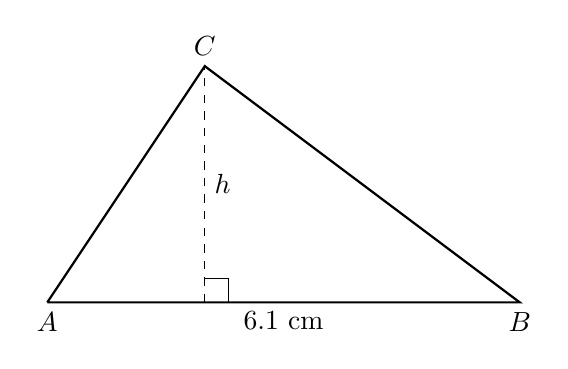
\begin{tikzpicture}%[scale=0.7]
     \draw [thick]
       (2,0)node[below]{$A$}--
       (8,0)node[below]{$B$}--
       (4,3)node[above]{$C$} --(2,0);
    \draw [dashed] (4,0)--(4,3);
    \draw (4,0)++(0.3,0)--++(0,0.3)--+(-0.3,0);
    \node at (4,1.5)[right]{$h$};
    \node at (5,0)[below]{$6.1$ cm};
  \end{tikzpicture} \vspace{2cm}

\item Find the volume of a pyramid ($V=\frac{1}{3}Bh$) having a height of 2 feet and with a square base having side lengths of 30 inches. Express your result to the \emph{nearest cubic foot}. \vspace{5cm}

\item Find the volume of a hemisphere with a radius of three inches, to the \emph{nearest whole cubic inch}. (The formula for the volume of a \emph{sphere} is $V=\frac{4}{3}\pi r^3$)

\newpage
\item A model rocket is in the shape of a cylinder with a cone-shaped nose cone on top. The diameter of both the cylindrical base and the nose cone is 3 inches. The cylinder section is 12 inches tall and the nose is an additional 3 inches in height. \\[0.5cm]
Find the volume of the rocket, using the formulas for a cylinder of $V=\pi r^2 h$ and a cone of $V=\frac{1}{3} \pi r^2 h$. Round the result to the \emph{nearest whole cubic inch}.  \vspace{8cm}

\item Given a rectangle with area 21, width $x$, and length $x+4$.
  \begin{enumerate}
    \item Find $x$. \vspace{4cm}
    \item Find the perimeter of the rectangle.
  \end{enumerate}

\end{enumerate}
\end{document}
